\chapter{Fundamentação Teórica}
\label{cap:fund}

%% - - - - - - - - - - - - - - - - - - - - - - - - - - - - - - - - - - -
\section{Aprendizado por Reforço}
\label{sec:rl}

O Aprendizado por Reforço (AR) é uma área do Aprendizado de Máquina que se concentra em como agentes de software devem tomar ações em um ambiente para maximizar alguma noção de recompensa cumulativa \cite{sutton}. 

\subsection{Conceitos Básicos}
\label{subsec:rl_conceitos}

O aprendizado por reforço é um paradigma computacional que explora como agentes podem aprender por meio da interação direta com o ambiente para alcançar objetivos específicos. Diferentemente de outros tipos de aprendizado, como o supervisionado e o não supervisionado, o aprendizado por reforço se baseia em um processo de tentativa e erro, no qual um agente busca maximizar um sinal de recompensa ao longo do tempo.

A interação entre o agente e o ambiente é representada esquematicamente na Figura \ref{fig/MDP.png}. O agente observa o estado atual \( S_t \) do ambiente e, com base em sua política de decisão, escolhe uma ação \( A_t \). Após a execução dessa ação, o ambiente evolui para um novo estado \( S_{t+1} \) e retorna ao agente uma recompensa \( R_{t+1} \) associada a essa transição.

\begin{figure}[h]
    \centering
    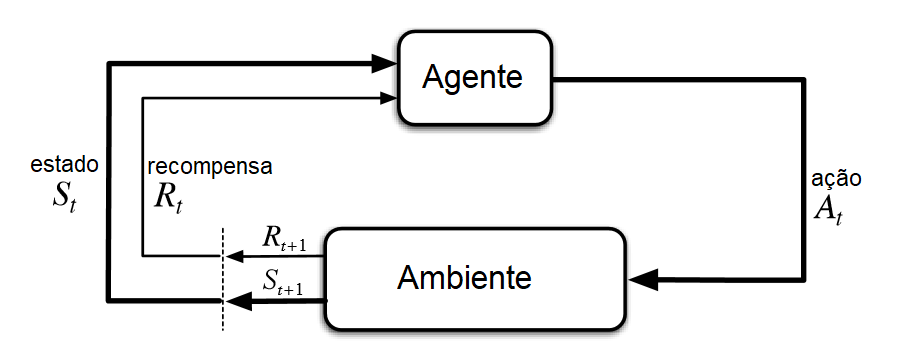
\includegraphics[width=0.6\textwidth]{fig/MDP.png}
    \caption{Interação agente-ambiente no aprendizado por reforço. O agente toma decisões com base no estado atual \( S_t \) e recebe do ambiente uma recompensa \( R_{t+1} \) após realizar a ação \( A_t \).}
    \label{fig:agent_env_interaction}
\end{figure}

\subsubsection*{Elementos Fundamentais:}
\begin{enumerate}
    \item \textbf{Agente e Ambiente:} O agente é a entidade responsável por tomar decisões, enquanto o ambiente é tudo aquilo que responde às ações do agente e fornece feedback.
    \item \textbf{Política (\(\pi\)):} Define a estratégia do agente, especificando a probabilidade de selecionar uma ação específica \( A_t \) em um estado \( S_t \).
    \item \textbf{Sinal de Recompensa (\(R_{t+1}\)):} Indica o valor imediato recebido pelo agente após realizar uma ação. O objetivo é maximizar a soma acumulada das recompensas ao longo do tempo.
    \item \textbf{Função de Valor (\(v(s)\) e \(q(s, a)\)):} Estima o valor esperado da recompensa futura a partir de um estado \( s \) ou de um par estado-ação \( (s, a) \).
\end{enumerate}

\subsubsection*{Exploração vs. Exploração:}
Uma característica central do aprendizado por reforço é o dilema entre explorar novas ações para adquirir conhecimento e explorar o conhecimento atual para maximizar recompensas. O equilíbrio correto entre esses dois aspectos é essencial para o sucesso do agente.

\subsubsection*{Modelagem por Processos de Decisão de Markov (MDPs):}
Os MDPs oferecem uma base teórica rigorosa para a modelagem do aprendizado por reforço, formalizando o problema com base nas transições entre estados, nas ações tomadas e nas recompensas recebidas. Um processo de decisão de Markov é definido pela propriedade de Markov, segundo a qual a probabilidade de transição para o próximo estado depende apenas do estado atual e da ação executada, não dos estados anteriores.

A interação entre o agente e o ambiente representada na Figura \ref{fig/MDP.png} exemplifica essa estrutura de MDPs, na qual o aprendizado por reforço visa encontrar uma política ótima que maximize o valor esperado das recompensas acumuladas.

\subsection{PPO (Proximal Policy Optimization)}
\label{subsec:ppo}

\subsection{Multi-agent RL}
\label{subsec:marl}

\subsection{Self-play}
\label{subsec:self_play}

%% - - - - - - - - - - - - - - - - - - - - - - - - - - - - - - - - - - -
\section{Curriculum Learning}
\label{sec:curriculum}

\subsection{Conceitos fundamentais}
\label{subsec:curriculum_conceitos}

\subsection{Aplicações em RL}
\label{subsec:curriculum_rl}

\subsection{Estado da arte}
\label{subsec:curriculum_estado_arte}

\subsection{Vantagens e desafios}
\label{subsec:curriculum_vantagens_desafios}

%% - - - - - - - - - - - - - - - - - - - - - - - - - - - - - - - - - - -
\section{Futebol de Robôs}
\label{sec:futebol_robos}

\subsection{Visão geral}
\label{subsec:futebol_visao}

\subsection{Desafios específicos}
\label{subsec:futebol_desafios}

\subsection{Trabalhos relacionados}
\label{subsec:futebol_trabalhos}